\documentclass{article}

\usepackage{fancyhdr}
\usepackage{ragged2e}
\usepackage{graphicx}
\usepackage{caption}
\usepackage{geometry}
\usepackage{amsmath}
\usepackage{rotating}

\usepackage{listings}
\usepackage{color}

\definecolor{dkgreen}{rgb}{0,0.6,0}
\definecolor{gray}{rgb}{0.5,0.5,0.5}
\definecolor{mauve}{rgb}{0.58,0,0.82}

\lstset{frame=tb,
  language=Java,
  aboveskip=3mm,
  belowskip=3mm,
  showstringspaces=false,
  columns=flexible,
  basicstyle={\small\ttfamily},
  numbers=none,
  numberstyle=\tiny\color{gray},
  keywordstyle=\color{blue},
  commentstyle=\color{dkgreen},
  stringstyle=\color{mauve},
  breaklines=true,
  breakatwhitespace=true,
  tabsize=4
}

\setcounter{secnumdepth}{1}

\usepackage{chngcntr}
\counterwithin{figure}{section}

\renewcommand*{\thepage}{C\arabic{page}}

\pagestyle{fancy}
\lhead{ACME Robotics}
\chead{\#8367}
\rhead{\ifcontents Contents \else Week \thesection \fi}

\newif\ifcontents
\contentsfalse

\makeatletter
\renewcommand{\@seccntformat}[1]{}
\makeatother

\begin{document}

\subsection{Start learning new tools and software}
%!New members of the software team need to familiarize themselves with Java, Android Studio, and the FTC SDK.
Emma and Clara completed a Code Academy Tutorial to learn the basics of Java, the language that the FTC app is programmed in. Then, inheritance was worked on because it is a major concept within the FTC SDK. Knowing how to do this will make understanding the code of the robot easier. Afterwards, a PowerPoint was reviewed that showed how to use Android Studio to practice coding.  The PowerPoint also gave examples and explained various function meanings in-depth. A TeleOp program was then written afterwards. Emma and Clara then set up and worked on the Modern Robotics training modules to help learn how to use sensors. It is crucial to know how to do this because sensors will need to be used for the new tasks of the robot. TeleOp code was looked at as well, followed by a series of videos for more in depth information.

\subsection{Test VuMark identification and Vuforia/OpenCV integration}
%!Get basic tracking and recognition of the pictographs (Vuforia VuMarks) working and convert Vuforia preview frames into Mats for OpenCV processing.	
By copying and slightly modifying the Concept VuMark Identification sample in the SDK, Ryan was able to quickly get VuMark identification working. The Opmode was successfully able to track the VuMarks and report both the autonomous bonus cryptobox column and the location of the VuMark. After that, Ryan researched how to convert Vuforia ClosableFrames to OpenCV Mats. Using some of the code from last year, he was able to extract grayscale images. His first attempts to get RGB frames were frustratingly unsuccessful until he figured out that the command to generate RGB frames had to be issued after the rest of the preview had initialized. Once this was figured out, the images were all loaded properly and ready for custom processing. The software team has decided to use OpenCV to try to ascertain the position of the jewels in autonomous; this is Ryan's next goal. A screenshot of VuMark identification is shown in figure \ref{fig:vumark}.
\begin{figure}[h]
    \centering
    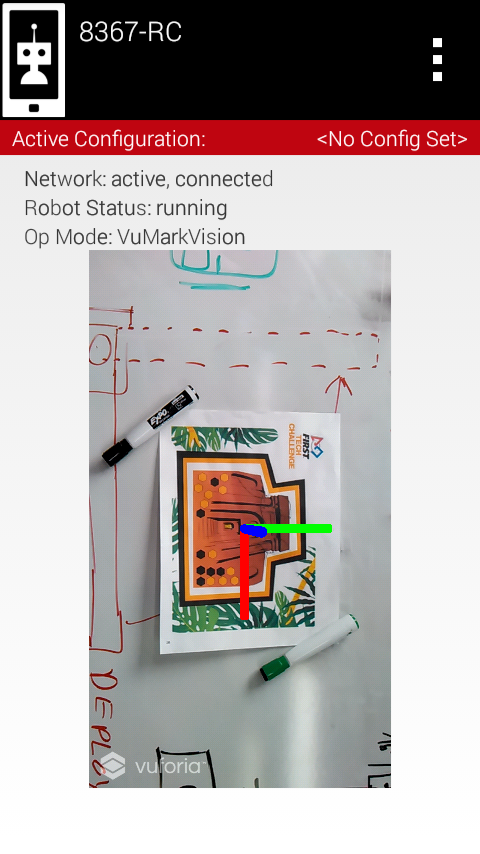
\includegraphics[width=.6\textwidth,height=3in,keepaspectratio]{01/images/vumark.png}
    \caption{Vuforia VuMark identification}
    \label{fig:vumark}
\end{figure}

\subsection{Explore options for cipher cube pattern assistance}
%!Explore the possibility of using software to intelligently choose what color glyph to pick up and where to put it, to make a pattern, as well as keep our options open.
In order to place the glyphs in patterns to correctly make the ciphers, scoring points, and allowing us to begin scoring a relic earlier, the process of choosing a color and where to place it had to be streamlined. Scenarios where it is only easy to pick up one color but there is nowhere for it to go drastically reduce the efficiency of glyph placement by forcing the robot to sort through the glyph pile. When the robot is able to choose between the two colors, the choice that maximizes future flexibility should be selected. The first idea was to use something similar to a minimax search algorithm, used for game playing algorithms. All the possible end states of the game are assigned a value, representing how desirable they are for one of the players. Then, working backward, it is assumed that the first player will always make the move that will maximize that value, and the other player, on their turn, will make the move that minimizes that value, an example of this is shown in figure \ref{fig:minimax}.
\begin{figure}[h]
    \centering
    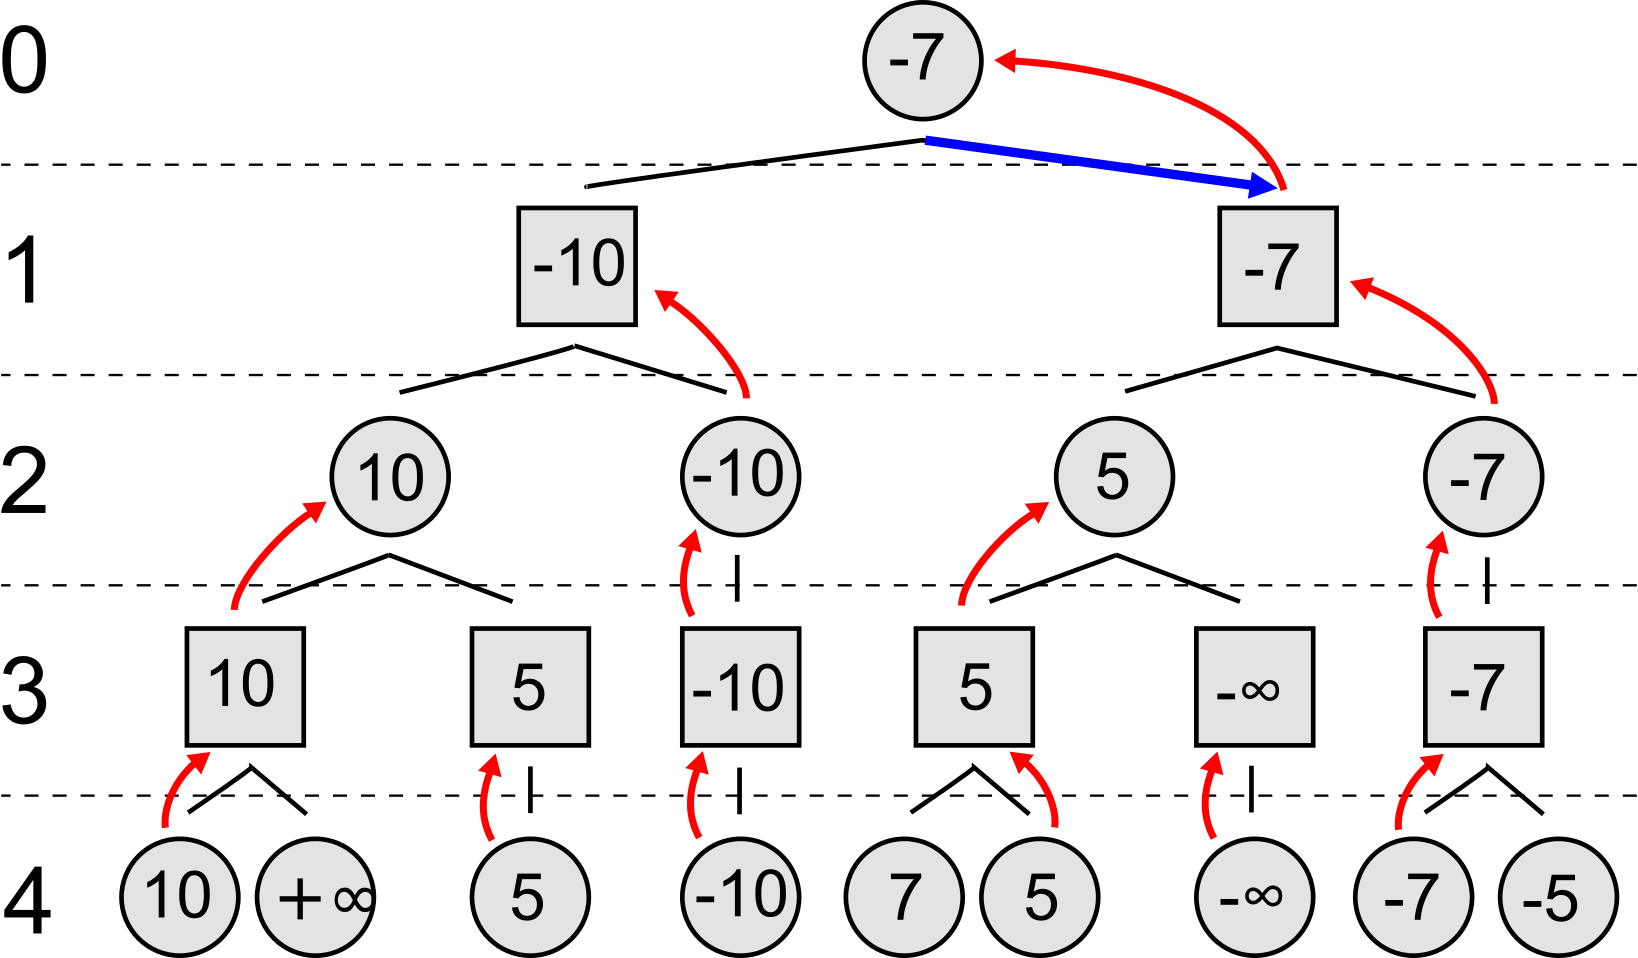
\includegraphics[width=.6\textwidth]{01/images/minimax.png}
    \caption{minimax algorithm}
    \label{fig:minimax}
\end{figure}
A similar algorithm could be applied to this problem, determining the flexibility afforded the robot at each possible state of the cipher cube, and then working backward, maximizing that flexibility at every decision, to decide what move to make to keep the most flexibility. Using this concept, the first attempt laid out all the possible cipher states in a tree. At the top is the initial configuration of the cipher, all empty. The children of each node are determined by enumerating all possible additions of a single cube, and then eliminating all states that cannot be made into a correct cipher. Each node was assigned a value of 0 if it was constraining, meaning that there is only one color of cube that could be added to the current state. To determine how desirable a node was the average value of all its children was taken. A higher number meant that, if that node was reached, the remaining cubes to be taken in and placed would be more flexible. This was a good representation of the flexibility of a state, but took a long time to run. With 12 moves, and 6 choices at each move (2 colors and 3 columns), there were $6^12$, or $2,176,782,336$ possible configurations of the cipher. One option to address this is to only search so deep into the tree. This greatly reduces the computational intensity. Another option is to come up with a function that estimates the desirability of a state.


\subsection{Brainstorm potential uses of software in the game}
%!Brainstorm potential uses for software control in both autonomous robot operation and driver assistance in teleop.
The software team analyzed different opportunities to use software to enhance the robot's capabilities in autonomous and teleop. In particular, we discussed methods for jewel identification and cryptobox alignment.	The software team brainstormed how effective software could be used in Relic Recovery to enhance the robot's performance. In autonomous, the two primary tasks are knocking the proper jewel and scoring glyphs in the cryptobox. For jewel identification, they discussed two potential methods, one using color sensors and another using vision. The color sensor initially seemed promising and hopefully simpler, but early tests revealed that the sensor had to be quite close to the jewel to get a reliable reading and not be pointing into one of the holes. In the end, the success of this method would largely depend on the orientation of the jewel and the consistency of the jewel manipulator/initial robot placement. The vision-based approach helps solve both these issues with the cost of some added complexity. Furthermore, the camera will already be pointed in the direction of the jewel stand to read the pictograph. After weighing the advantages and disadvantages of both approaches, the software team decided to pursue OpenCV-based color detection for jewel identification. For glyph scoring, the primary difficulty seems to be properly aligning with the cryptobox. Although dead reckoning from our starting position could work, it isn't very robust and errors accumulate quickly (especially if the robot makes multiple scoring runs in autonomous). Furthermore, it would be helpful to have similar alignment functionality in teleop to assist the drivers and score glyphs more quickly. Unfortunately, the pictographs aren't optimally placed for cryptobox alignment; there are none nearby the side/auxiliary box and they become occluded as the robot approaches the cryptobox. The only solution the team came up with was again using vision to detect the cryptobox and use its positioning in the image and the robot orientation from the IMU to align. Although rather complex and potentially unstable, this seems like the only solution that satisfies the requirements.

\end{document}